% \section{Aufbau und Durchführung}
\noindent Zum experimentellen Aufbau des Versuchs gehört eine
$^{137}Cs$-Strahlungsquelle, welche in eine Absorbierende Ummantelung aus Blei
geschraubt wird. Neben der Quelle befindet sich in Durchlassrichtung für den
Strahl aus Gammaphotonen ein drehbarer Probenhaltertisch, welcher mittels einer
Stellschraube in den Strahlengang hinein und daraus hinaus geschoben werden
kann. Daneben, am Ende des Strahlengangs ist ein $NaJ$-Detektor positioniert,
welcher die am Detektor ankommende Intensität der Gammaphotonen registriert.
Abschließend folgt eine weitere Bleiabschirmung. \\
\noindent Die Probe selbst ist ein Würfel der Kantenlänge $\SI{3}{\centi\meter}$
und besteht aus insgesamt 27 kleineren Würfeln. Seine Wandstärke beträgt etwa
$\SI{1}{\milli\meter}$ und besteht aus Aluminium. \\
\FloatBarrier
\begin{figure}
  \centering
  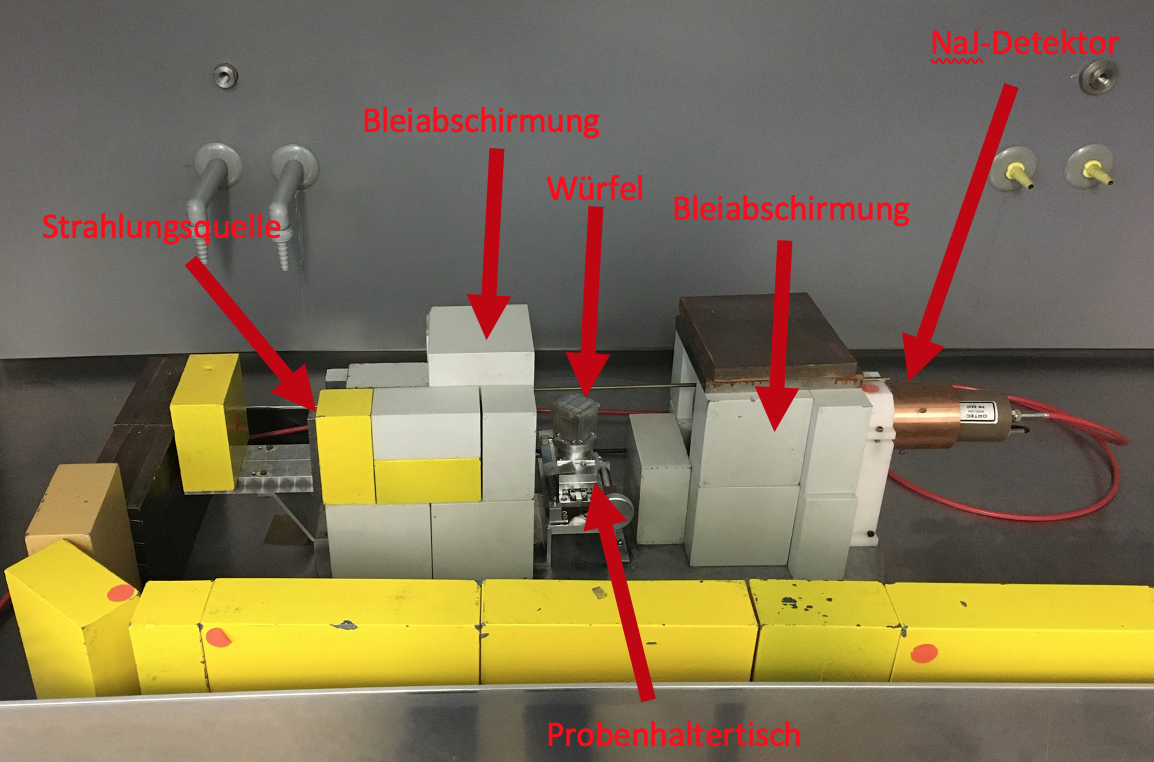
\includegraphics[scale=0.5]{ressources/aufbau.png}
  \caption{Versuchsaufbau zur Tomographie mit Gammastrahlung.}
  \label{fig:03}
\end{figure}
\FloatBarrier
\noindent Untersucht werden soll die Zusammensetzung der mittleren Schicht von
vier verschiedenen Würfeln der oben genannten Abmaße. Dazu wird die Probe
mithilfe einer Schraube auf dem Probenhaltertisch fixiert und aus insgesamt
zwölf verschiedenen Richtungen gemäß Abbildung \ref{fig:04} durchstrahlt.
\FloatBarrier
\begin{figure}
  \centering
  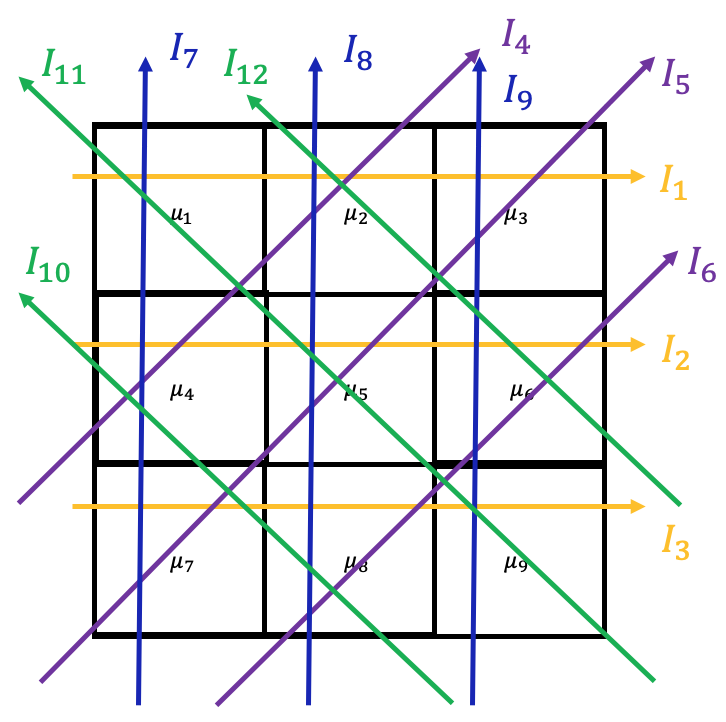
\includegraphics[scale=0.5]{ressources/strahlengang.png}
  \caption{Theoretischer Strahlengang dirch die mittlere Ebene des Würfels.}
  \label{fig:04}
\end{figure}
\FloatBarrier
\noindent In ihrer Intensität verringert treffen die Gammaphotonen auf den
Szintillationsdetektor. Dort werden mithilfe des Photoeffekts Elektronen
aus dem Detektormaterial herausgelöst und zwischen Dynoden, an welchen eine
Spannungskaskade anliegt beschleunigt und vervielfältigt. Das ausgehende Signal
ist dabei proportional zum Eingangssignal von Gammaphotonen. \\
\noindent Zu beginn der Messung wird ein hohler Aluminiumwürfel gemessen, um die
Nullrate der Gammaphotonen bestimmen zu können. Die Messzeit beträgt je Richtung
mindestens fünf Minuten. Die Dauer korelliert dabei mit der Anzahl der Gemessenen
Photonen. Um statistische Messungenauigkeiten auf ein verträgliches Niveau zu
bringen, gilt für die Anzahl an registierten Gammaphotonen
\begin{align}
  \frac{1}{\sqrt{N}} < \num{0.03},
\end{align}
\noindent wobei der Wert $\num{0.03}$ dabei als $\SI{3}{\percent}$ Grenze für
die Messungenauigkeit aufzufassen ist. Die Anzahl der zu registrierenden
Ereignisse liegt daher bei etwa $\num{1100}$ und sollte innerhalb der
fünfminütigen Messzeit erreicht werden. Falls dies nicht der Fall ist, ist eine
Anpassung der Messzeit erforderlich. \\
